\documentclass{article}
\usepackage{graphicx}
\usepackage{enumerate}
\usepackage{setspace}
\usepackage{hyperref}
\usepackage[utf8]{inputenc}
\usepackage[OT1]{fontenc}
\usepackage[french]{babel}
\usepackage{vmargin}
\setpapersize{A4}
\setmargins{15mm}{15mm}{180mm}{260mm}{0pt}{0mm}{0pt}{1.2cm}
\title{Compte rendu OUTILS LIBRES}
\author{REVEL Rémi}
\date{\today}

\begin{document}
\maketitle
\par\noindent\rule{\textwidth}{0.4pt}

\section{\huge{efficatité de l'environnemnt de travail}}
%----------------------------------------Question 1-----------------------------------------------------
\subsection{\large{Desactivation de la souris}}

\subsection*{\normalsize{voici les commande pour desactiver la souris:} } 
\begin{enumerate}
    \item xinput set-prop 4 "Device Enabled" 0

    \item xinput set-prop 6 "Device Enabled" 0

    \item xinput set-prop 7 "Device Enabled" 0
\end{enumerate}

\subsection*{\normalsize{tableau de raccourcis clavier utile:} }    

\begin{center}
   \begin{tabular}{| l | c | }
     \hline
     changer d'application & alt+tab ou windows+tab\\ \hline
     gestionnaire d'application & Touche windows \\ \hline
     Naviguer sur les elements cliquable d'une page web & tab   \\ \hline
     Fermer le navigateur & CTRL+W \\ \hline
     Fermer une appliacation & ALT+F4 \\ \hline
     Changer d'onglet sous Brave & CTRL+1,2,3,...   \\ \hline
     Ouvrir un nouvelle onglet & CMD+T \\ \hline
     faire une recherche & F6 \\ \hline
   \end{tabular}
 \end{center}
 
 %---------------------------------------------------------------------------------------------
 
 %----------------------------------------question 2-----------------------------------------------------
 \subsection{\large{S'ameliorer a la dactylographie}}
 le site que j'ai retenu pour s'ameliorer en dactylographie est \href{https://10fastfingers.com/typing-test/french}{10fastfingers}. \par On peut s'entrainer sur des mots aleatoire, ou sur nos propres texte, le site est disponible dans plusieurs langue.

\begin{center}
    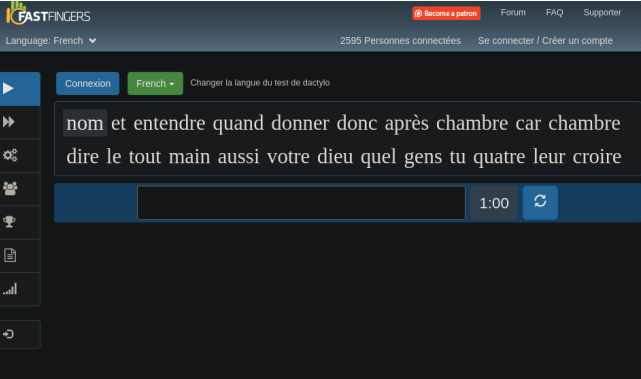
\includegraphics[scale=0.7]{Images/fastfinger.png}
\end{center}

%---------------------------------------------Question 3------------------------------------------------

\end{document}
